\documentclass{template/openetcs_report}
% Use the option "nocc" if the document is not licensed under Creative Commons
%\documentclass[nocc]{template/openetcs_report}
\usepackage{lipsum,url}
\usepackage{supertabular}
\usepackage{multirow}
\usepackage{color, colortbl}
\definecolor{gray}{rgb}{0.8,0.8,0.8}
\usepackage[modulo]{lineno}
\usepackage{hyperref}
\usepackage{listings}
\usepackage{makeidx}
\makeindex
\graphicspath{{./template/}{.}{./images/}}

\newcommand{\define}[1]{\index{#1}\emph{#1}}

\begin{document}
\frontmatter
\project{openETCS}

%Please do not change anything above this line
%============================
% The document metadata is defined below

%assign a report number here
\reportnum{OETCS/WP3/D??}

%define your workpackage or task here
\wp{openETCS@ITEA Work Package 3: ``Modelling''}

%set a title here
\title{openETCS API description}

%set a subtitle here
\subtitle{Generic interface between openETCS application and overall system}

%set the date of the report here
%\date{August 2012\\Revised May 2014}
\date{June 2014}

%document approval
%define the name and affiliation of the people involved in the documents approbation here
\creatorname{[creator name]}
\creatoraffil{[affiliation]}

\techassessorname{[assessor name]}
\techassessoraffil{[affiliation]}

\qualityassessorname{[assessor name]}
\qualityassessoraffil{[affiliation]}

\approvalname{Klaus-R\"udiger Hase}
\approvalaffil{DB Netz}

%define a list of authors and their affiliation here
\author{Nicolas Boverie}

\affiliation{Alstom Transport}

\author{David Mentré}

\affiliation{Mitsubishi Electric R\&D Centre Europe}

\author{Nicolas Van Landeghem}

\affiliation{ERSA}

% define the coverart
\coverart[width=350pt]{openETCS_EUPL.png}

%define the type of report
\reporttype{Draft Report}


\begin{abstract}
%define an abstract here
  FIXME
\end{abstract}

%=============================
%Do not change the next three lines
\maketitle

%Modification history
%if you do not need a modification history table for your document simply comment out the eight lines below
%=============================
\section*{Modification History}
\tablefirsthead{
\hline 
\rowcolor{gray} 
Version & Section & Modification / Description & Author \\\hline}
\begin{supertabular}{| m{1.2cm} | m{1.2cm} | m{6.6cm} | m{4cm} |}
 & & & \\\hline
\end{supertabular}

\tableofcontents
\listoffiguresandtables

%=============================
%Uncomment the next line if you need line numbers for tracebility when the document is in review
%\linenumbers

%=============================
% The actual document starts below this line
%=============================

%Start here


\mainmatter

%Examples are below

\chapter{Introduction and context}

\section{Introduction}

This document describes the ``openETCS API''. The openETCS API is an
open, standardized, interface between a vendor specific platform and
the openETCS application software. More details on the software
architecture are given in chapter \ref{software-arch}.

\paragraph{Main objectives} The main objectives of this document are
to describe an API:
\begin{itemize}
\item Suitable for every partner of openETCS project;
\item Compatible with Vendor specific API through an ``Adaptation Layer'';
\item Making explicit all assumptions, including non-functional ones;
\item Language agnostic, allowing interfacing with software written
  in C, Ada or other programming languages;
\item Simple;
\item Fulfilling safety objectives;
\item Offering reasonable performance.
\end{itemize}


\section{References}

The requirements for this document are defined in \cite[§7.1]{D2.6-9} and
\cite{API-req-2} documents.

Source of information and constraints for this document are following
documents:
\begin{itemize}
\item Alstom API proposal defined in \cite{alstom-api},
  \cite{alstom-api-app-layer} and \cite{alstom-api-data-dict};
\item Comments on Alstom API proposal in \cite{alstom-api-comments};
\item The top level interfaces of \cite{sysml-model};
\item SCADE openETCS model requirements on run-time defined in §2.2
  and §3 of \cite{scade-modelling-guide};
\item ERSA Simulator API \FIXME{ref??} %%\cite{??};
\item ETCS on-board interfaces as pointed out in Figure 1 of §2.5.3 in
  \cite{subset-026}.
\end{itemize}


\section{Identified issues}

This documents aims at reaching a consensus, satisfying relevant point
of view of all openETCS project's partners.

As of now, we have identified following issues on which no consensus
has been found (yet!):
\begin{enumerate}
\item Timing requirements are currently incompatible between SCADE
  model and Alstom's API definition
  \begin{enumerate}
  \item 	Sub-issue regarding cycle time definition
  \item 	Sub-issue regarding ordering of events
  \end{enumerate}
\item The data flow definition in Alstom's API proposal is sometimes
  too far from SRS
\item No agreement on the overall behaviour of Basic software and
  Application software: when data flows are exchanged, how they are
  stored, constraints on them, ...
  \begin{enumerate}
  \item No agreement on general software architecture
  \item What is in application Sw and generic software?
  \end{enumerate}
\item Define what is in or out of application (odometry, crc, ...)?
  Allow differentiation points between suppliers
\item No agreement on the way the various components are calling each
  other: order sequence, constraints, ...
\item How to manage physical units in unambiguous way?
\item The API description should distinguish abstract and concrete
  parts:
  \begin{enumerate}
  \item Abstract parts: Dataflows, Datatypes, Input/Output, ...
  \item Concrete parts: Given by value or reference, C or Ada
    language, where is made allocation and (possible) de-allocation,
    ...
  \end{enumerate}
\end{enumerate}

\section{Abbreviations}

Abbreviations not described in this section are described in
\cite{subset-023}.

\begin{description}
\item[\define{API}] Application Programming Interface. An interface
  between two parts of a system, describing aspects that the two parts
  shall be compliant with and keeping other points undetermined
\item [\define{BIU}] \FIXME{def??}
\item [\define{JRU}] Juridical Recording Unit
\end{description}

% LocalWords:  Alstom API openETCS SysML


\chapter{Reference abstract hardware architecture}

\section{Why a reference abstract hardware architecture?}

For proper understanding of openETCS API and of constraints imposed on
both sides of the API, we need to define a \emph{reference abstract
  hardware architecture}. This hardware architecture is ``abstract''
is the sense that the actual vendor specific hardware architecture
might be totally different of the abstract architecture described in
this chapter. For example, several units might be grouped together on
the same processor.

However the actual vendor specific architecture shall fulfill all the
requirements and constraints of this reference abstract hardware
architecture and shall not request additional constraints.

\section{Definition of the reference abstract hardware architecture}

\begin{figure}
  \centering
  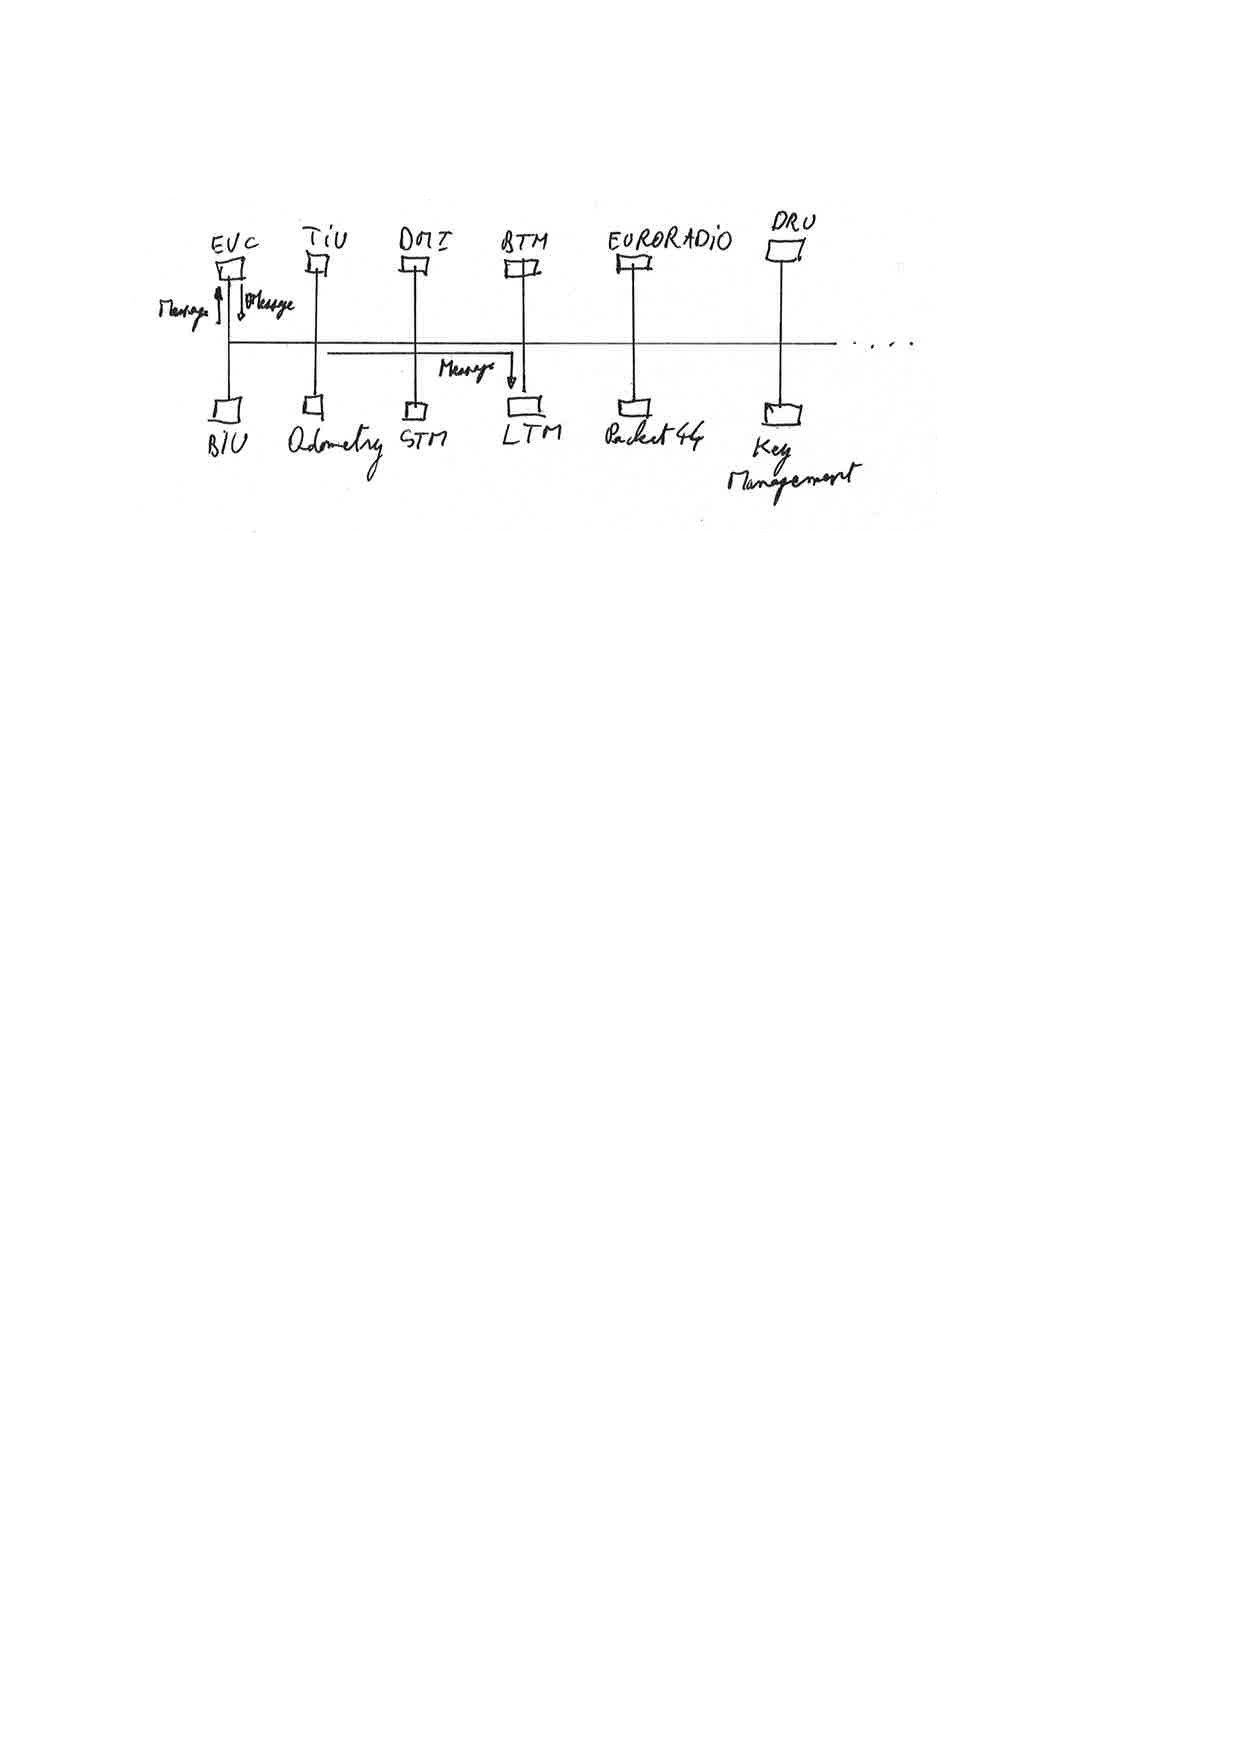
\includegraphics{abstract-hardware-architecture.pdf}
  \caption{Reference abstract hardware architecture}
  \label{fig:hardware-arch}
\end{figure}

The reference abstract hardware architecture is shown in figure
\ref{fig:hardware-arch}.

The reference abstract hardware architecture is made of a bus on which
are connected physical units:
\begin{itemize}
\item EVC (European Vital Computer);
\item BIU \FIXME{def??};
\item TIU (Train Interface Unit);
\item Odometry;
\item DMI (Driver Machine Interface);
\item STM (Specific Transmission Module);
\item BTM (Balise Transmission Module);
\item LTM (Loop Transmission Module);
\item EURORADIO;
\item JRU (Juridical Recording Unit);
\item Packet 44 (Alstom Transport specific module, \cite{alstom-api});
\item DRU (Diagnostic Recording Unit, Alstom Transport specific
  module, \cite{alstom-api});
\item Key Management (Alstom Transport specific module,
  \cite{alstom-api});
\item Other units.
\end{itemize}

A given instance of openETCS might not have all of above
units. \FIXME{Define a set of mandatory units?}

Those units shall working concurrently. They shall exchange
information with other units through asynchronous message passing.

% LocalWords:  Alstom openETCS EVC BIU TIU Odometry DMI STM BTM Balise LTM API
% LocalWords:  EURORADIO JRU


\chapter{Reference abstract software architecture}
\label{software-arch}

\begin{figure}[htbp]
  \centering
  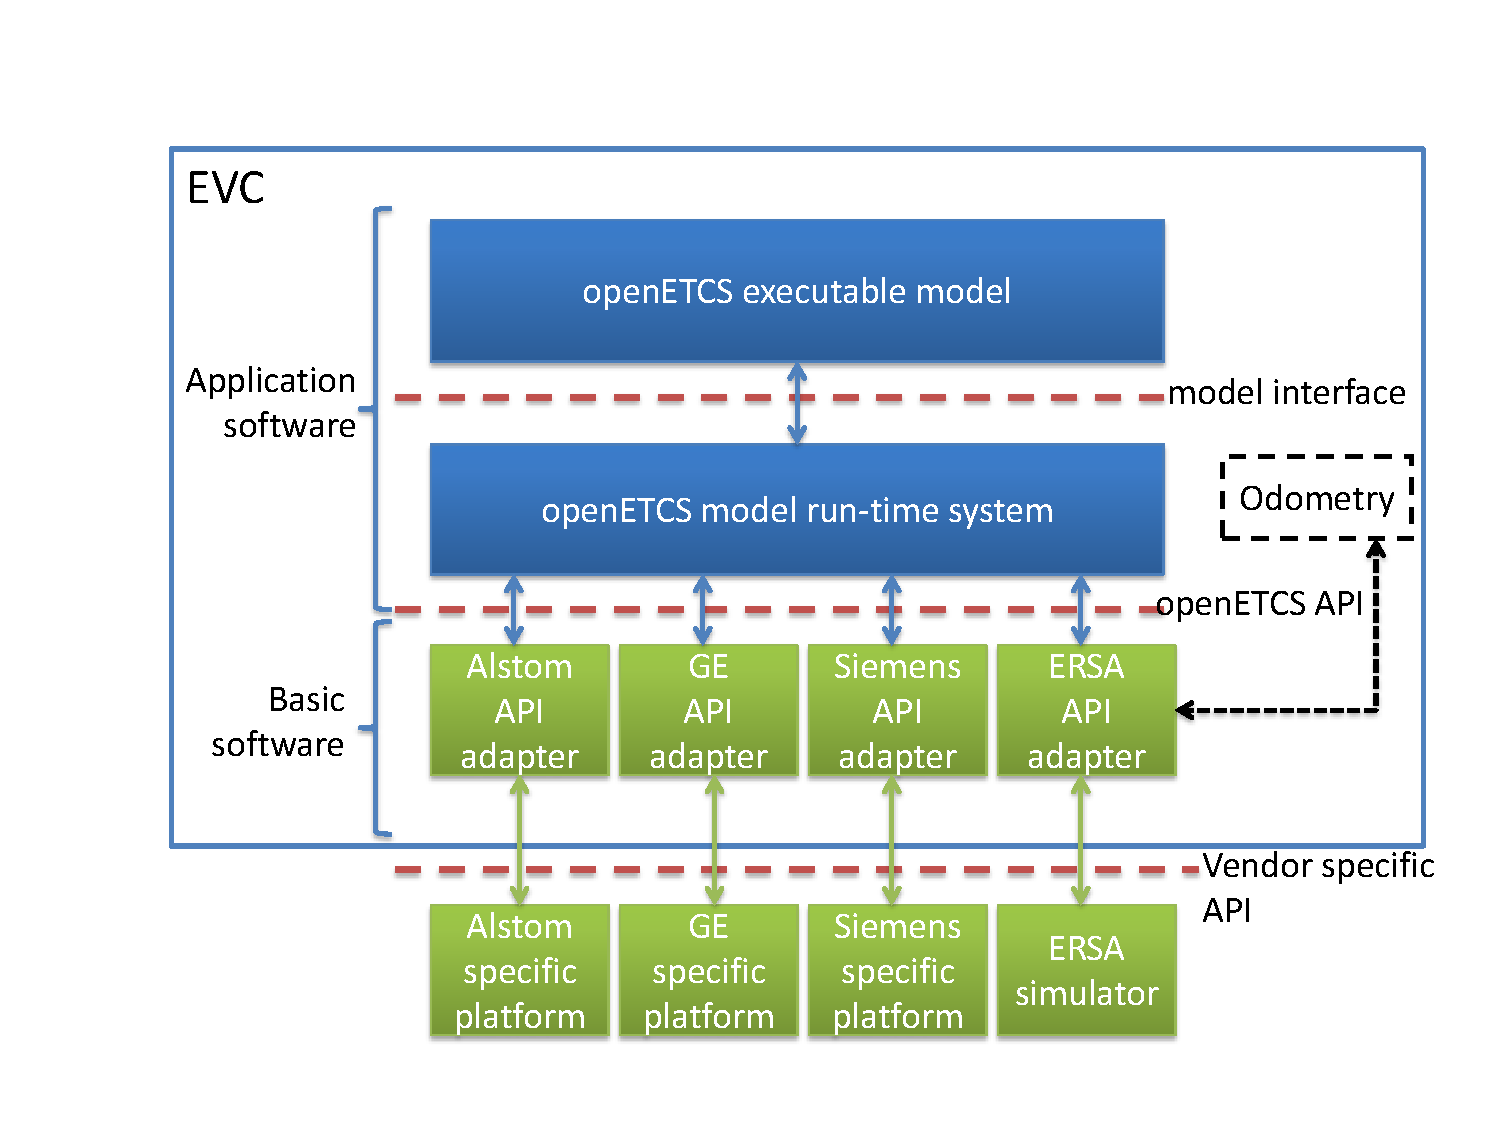
\includegraphics[width=\linewidth]{software-architecture.pdf}
  \caption{Reference abstract software architecture}
  \label{fig:software-arch}
\end{figure}

The \emph{reference abstract software architecture} is shown in figure
\ref{fig:software-arch}. This architecture is made of following
elements:
\begin{itemize}
\item \emph{openETCS executable model} produced by the
  \cite{scade-model}. It shall contain the program implementing core
  ETCS functions;
\item \emph{openETCS model run-time system} shall help the execution
  of the openETCS executable model by providing additional functions
  like encode/decode messages, proper execution of the model through
  appropriate scheduling, re-order or prioritize messages, etc. This
  block shall be described in another openETCS document. \FIXME{ref?}
\item \emph{Vendor specific API adapter} shall make the link between
  the Vendor specific platform and the openETCS model run-time system.
  It can buffer message parts, encode/decode messages, route messages
  to other EVC components, etc.
\item All above three elements shall be included in the EVC;
\item \emph{Vendor specific platform} shall be all other elements of
  the system, bus and other units, as shown in figure
  \ref{fig:hardware-arch}.
\end{itemize}

We have thus three interfaces:
\begin{itemize}
\item \emph{model interface} is the interface between openETCS
  executable model and openETCS model run-time system. It shall be
  described in another openETCS document \FIXME{ref?};
\item \emph{openETCS API} is the interface between openETCS model
  run-time system and Vendor specific API adapter. It is described in
  this document;
\item \emph{Vendor specific API} is the interface between Vendor
  specific API adapter and Vendor specific platform. This interface is
  not publicly described.
\end{itemize}

The two blocks openETCS executable model and openETCS model run-time
system are making the \emph{Application software} part.

The Vendor specific API adapter is making the \emph{Basic software}
part.

\paragraph{Information exchange between blocks}
At this level of description, we do not explain how the various blocks
of above architecture are calling themselves. We only assume they are
exchanging \emph{messages} in an asynchronous way. A message is a set
of information corresponding to an event of a particular unit, e.g. a
balise received from the BTM. The possible kind of messages are
described in chapter \ref{information-flows}.

How the exchange of messages in implemented in actual software,
e.g. function call, storage of data in a shared buffer, ..., is
described in chapter \ref{concrete-interface}.

\paragraph{Architectural variations}
Please note that the reference abstract hardware and software
architectures do not forbid architectural variations. For example, the
Odometry function could be put within the EVC (see figure
\ref{fig:software-arch}) instead of a separate hardware unit (as it
was shown on figure \ref{fig:hardware-arch}). Such Odometry function
would be part of the Application software. But communication between
this Odometry function within EVC and the openETCS model run-time
system should be done through the openETCS API and follow its
conventions.

As another example, part of Vendor specific platform could be on EVC
and thus the Vendor specific API would be within the EVC.


% LocalWords:  openETCS API EVC Odometry balise BTM


\chapter{Real-time and ordering constraints}

For proper functioning of the system, the openETCS API specifies
real-time and ordering constraints that both the Application software
as well as the Basic software and remaining of the system shall
ensure. Those constraints are described in this chapter.

Overall, those constraints shall ensure the ETCS Requirements on
performance (\cite{subset-041}) are fulfilled. Some of those
constraints are coming from Alstom Transport (\cite{alstom-api}).

\section{Cyclic execution of the Basic and Application software}

Both Basic and Application software shall be initialized once, in an
\define{initialization phase}, and then shall be executed cyclically
in a sequence of \define{cycles}.

During initialization phase, all units of the system shall be
initialized and be ready to proceed at the end of initialization
phase.

\section{Ordering constraints on message exchange}
\label{sec:ordering-constraints}

Between units of the system (DMI, EVC, ...), following constraints
shall be ensured:
\begin{itemize}
\item No message shall be lost;
\item Messages sent from one unit towards another one shall be
  received in emission order;
\item Messages sent from two units towards a
single one or received by a single units from two other units shall be
received in any order.
\end{itemize}

\section{Real-time constraints}

\subsection{Event propagation delay}
\label{sec:event-propagation-delay}

The \define{external world} is the physical world out of the ETCS
system. This external world sends and receives \define{events} to/from
the ETCS system.

When an external world event is seen on a unit of the system
(e.g. balise received in BTM), this event is processed and a message
might be sent to another unit (e.g. EVC). In the reverse, a unit
(e.g. EVC) might send a message to another unit (e.g. DMI) that might
produce an event to the external world (e.g. display a message to the
driver).

The system shall ensure following constraints:
\begin{itemize}
\item The minimum delay from an input event received of the external
  world until it is received (in a message) by the Application
  software shall be \FIXME{XX ms};
\item The maximum delay from an input event of the external world
  until it is received (in a message) by the Application software
  shall be \FIXME{XX ms};
\item The minimum delay from a message sent by the Application
  software until an event is sent to the external world shall be
  \FIXME{XX ms};
\item The maximum delay from a message sent by the Application
  software until an event is sent to the external world shall be
  \FIXME{XX ms}.
\end{itemize}

\subsection{Event re-ordering}

As a consequence of ordering constrains on message exchange
(§\ref{sec:ordering-constraints}) and event propagation delay
(§\ref{sec:event-propagation-delay}), two messages corresponding to
two events (e.g. reception of a balise and a radio message) on two
different units (e.g. BTM and EURORADIO) send towards a third unit
(e.g. EVC) might not be received in real time order, i.e. the message
corresponding to the first real time event might arrive in second
position on the reception unit.

\subsection{Event time-stamping}

The system is asynchronous: an event is received on a unit and some
time is spent before seeing the corresponding message in another
unit. In order to do its computations, the Application software needs
to know at which real time the event was received. In order to do so,
a time-stamp shall be applied on all events requiring such
computations. \FIXME{Make a list of such events?}

This time-stamp shall fulfill
following constraints:
\begin{itemize}
\item Time-stamp clock shall have a precision of 1 µs, with a
  deviation compared to real time of less than 0.1\%;
\item Time-stamp clock shall be the same on all units of the system.
\end{itemize}

\subsection{Execution time constraints}

The following real-time constrains shall be ensured:
\begin{itemize}
\item The maximum execution time taken by Application software for
  initialization step is 100 ms;
\item The maximum execution time of the Basic and Application software
  in a cycle shall be \FIXME{300 + XX ms};
\item The maximum execution time of the Application software in a
  cycle shall be 100 ms.
\end{itemize}

\section{Event burst}

In some situation, a burst of events can occur. The following
dimensioning shall be ensured:
\begin{itemize}
\item The maximum number of event sent by a unit shall be at most
  \FIXME{XX events};
\item The maximum number of event received by a unit shall be at most
  \FIXME{XX events}.
\end{itemize}

\FIXME{Do we need to define the total number of events?}

\FIXME{Do we need to define what to do when those maximums are
  reached?}

% LocalWords:  openETCS DMI EVC API ETCS Alstom BTM balise EURORADIO


\chapter{Abstract information flows}
\label{information-flows}

We describe in this chapter the information flow betwen EVC and other
units using ASN.1 notation. See appendix \ref{asn1-primer} to know
more about ASN.1.

\section{Train Interface}

The interface between the EVC and Train Interface Unit is defined in
following \ASN{Train-interface} module. This module defines
\ASN{Message-Train-Interface-to-EVC} and
\ASN{Message-EVC-to-Train-Interface}.

\lstinputlisting[language=ASN1]{asn1/train-interface.asn}


\chapter{Concrete interface with openETCS model}
\label{concrete-interface}


\bibliographystyle{klunamed}
\bibliography{api-description}

\printindex

%===================================================
%Do NOT change anything below this line

\end{document}
